\documentclass[12pt,a4paper]{article}

% === PAQUETES === (((
\usepackage{amsmath}
\usepackage[shortlabels]{enumitem}
\usepackage{amsfonts}
\usepackage{ragged2e}
\usepackage{subfigure}
\usepackage{amssymb}
\usepackage{slashbox}
\usepackage{multirow}
\usepackage{multicol}
\usepackage{fontspec}
\usepackage{fullpage}
\usepackage{graphicx}
\usepackage{titlesec} 
% \usepackage{setspace}
\usepackage{dsfont}
% \usepackage{bookmark}
% )))

% === TIPOGRAFÍA === (((
\setmainfont[
  BoldFont       = bodonibi,
	ItalicFont     = Century modern italic2.ttf,
	BoldItalicFont = bodonibi,
	SmallCapsFont  = lmromancaps10-regular.otf
]{Century_modern.ttf}
% )))

% === COMANDOS === (((
\newcommand{\dis}{\displaystyle}
\newcommand{\qed}{\hspace{0.5cm}\rule{0.16cm}{0.4cm}}
\newcommand{\micita}[1]{\([\)\cite{#1}\(]\)}
\newcommand{\operator}[1]{\mathop{\vphantom{\sum}\mathchoice{ \vcenter{\hbox{\huge $#1$}} }
{\vcenter{ \hbox{\Large $#1$}} }{#1}{#1}}\displaylimits}
\newcommand{\suma}{\operator{ 
\includegraphics[scale=0.09]{IMAGENES/Sigma.png}} }
\DeclareSymbolFont{italics}{\encodingdefault}{\rmdefault}{m}{it}
\DeclareSymbolFontAlphabet{\mathit}{italics}
\ExplSyntaxOn
\int_step_inline:nnnn { `A } { 1 } { `Z }
 {  \exp_args:Nf \DeclareMathSymbol{\char_generate:nn{#1}{11}}{\mathalpha}{italics}{#1} }
\int_step_inline:nnnn { `a } { 1 } { `z } {  \exp_args:Nf \DeclareMathSymbol{\char_generate:nn{#1}{11}}{\mathalpha}{italics}{#1}}
\ExplSyntaxOff
% )))

% === SECCIONES === (((
\titleformat*{\section}{\large\normalfont\bfseries}
\titleformat*{\subsection}{\large\itshape \centering}
% \setcounter{secnumdepth}{0}
\renewcommand*{\contentsname}{\large\textbf{CONTENIDOS.}}
\usepackage[nottoc,numbib]{tocbibind}
\renewcommand{\refname}{REFERENCIAS.}
\renewcommand{\tablename}{Tabla}
\renewcommand{\figurename}{Figura}
% )))

% === PORTADA === (((
% \pagestyle{empty}
\newcommand{\portada}{
\addfontfeature{LetterSpace=-5}
  \begin{titlepage}
  \centering
  \begin{figure}
    \centering
    
\includegraphics[scale=0.5]{IMAGENES/logo_uaa.png}  
  \end{figure}
  {\bfseries\Large\MakeUppercase{\textit{Universidad Autónoma de Aguascalientes.}} \par}
  \vspace{1cm}
  {\Large Centro de Ciencias Básicas. \vspace{0.5cm}\\[2mm]
  Departamento de Matemáticas y Física.\vspace{0.5cm}\\[2mm]
  Licenciatura en Matemáticas Aplicadas.\vspace{0.5cm}\\[2mm]
  Práctica 6.\par}
  \vspace{1.5cm}
  {\bfseries\Huge Experimento de Young. \par} % title
  \vspace{1.5cm}
  {\itshape\Large Óptica. \\Prof. Mariana Alfaro Gómez.\par}
  % {\itshape\Large Variable Compleja I. \\Prof. Fausto Arturo Contreras Rosales.\par}
  % {\itshape\Large Métodos Numéricos II. \\Prof. Manuel Ramírez Aranda.\par}
  % {\itshape\Large Diseño de Experimentos. \\Prof. Angélica Hernández Quintero.\par}
  % {\itshape\Large Filosofía de la Investigación Científica. \\Prof. Jesús Mariano Rodríguez Muñoz.\par}
  \vfill
  % {\Large \textit{Por Erick I. Rodríguez Juárez.}\par}
		\begin{flushleft}
		\Large
		Alumnos:\\
		\textit{Carlos Francisco Guzmán Barba.}\\
		\textit{Erick Ignacio Rodríguez Juárez.}\\
		\textit{Manuel Alejandro Siller Landin.}
		\end{flushleft}
	% {}  % {\Large \textit{Por Erick I. Rodríguez Juárez.}\par}
  \vfill
		\begin{flushright}
		{\Large Realización: 2\(/\)05\(/\)22. \par} % date
		{\Large Entrega: 16\(/\)05\(/\)22. \par} % date
		\end{flushright}
  \end{titlepage} 
	% \thispagestyle{empty}
	% \doublespacing
	% \tableofcontents
	% \singlespacing
	% \newpage
} 
% )))

\begin{document}

\portada

\section{RESUMEN.} % (((
% )))

\section{INTRODUCCIÓN.} % (((
Si el ángulo es pequeño, entonces el \(OPQ\) es semejante a \(S_1S_1 \delta\).
\begin{figure}[hbtp!]
	\centering
	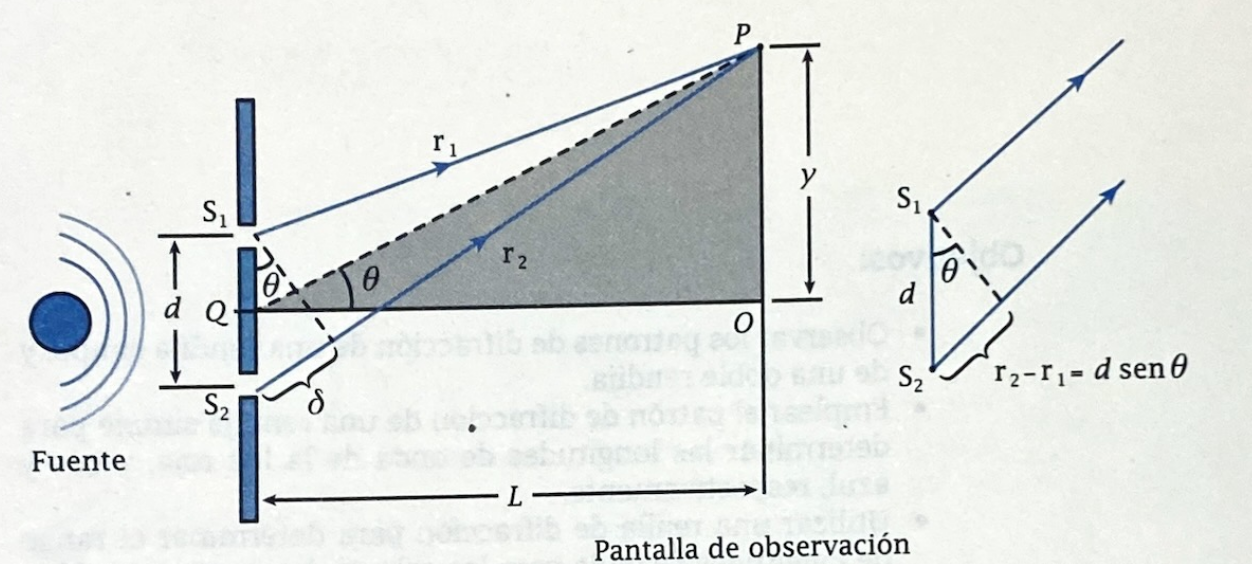
\includegraphics[width= 0.8 \linewidth]{1_INTRO/geometria.png}
	\caption{Experimento de la Doble Rendija de Young.}
	\label{fig:constructiva}
\end{figure}\\
La interferencia es constructiva siempre que \(r_1-r_2 = m \lambda\), para algún \(m \in \mathds{Z}\). Es decir
\begin{equation}
	d \sin \theta = m \lambda , \hspace{1cm} m \in \mathds{Z} .
	\label{eq:young}
\end{equation}
donde se alcanzará un máximo cuando \(m \in \mathds{Z}\). Y si \(m=k/2\), con \(k\) impar, entonces se alcanzará un mínimo. Además, el campo eléctrico \(E_i\) en el punto \(S_i\) está dado por
\begin{equation}
	\begin{array}{rcl}
		E_1 & = & E_0 \sin wt \\[2mm]
		E_2 & = & E_0 \sin (wt+ \phi)
	\end{array}
	\label{eq:campos_electricos}
\end{equation}
Y por el principio de superposición, tendremos que el campo eléctrico total es:
\begin{equation}
	E = E_1 + E_2 = (2E_0 \cos \beta) \sin (wt+ \beta).
	\label{eq:campo_total}
\end{equation}
donde \(\beta = \phi /2\). Recordamos que \(\beta = \dfrac{2 \pi \sin \theta}{\lambda}\), y la intensidad para el ángulo \(\theta\) está dada por
\begin{equation}
	I(\theta) = 4I_0 \cos ^2 \beta = 4I_0 \cos ^2 \bigg(\dfrac{\pi d \sin \theta}{\lambda}\bigg).
	\label{eq:intensidad}
\end{equation}
Los máximos son alcnazados cuando
\begin{equation}
	W \sin \theta = n \lambda , \hspace{1cm} n \in \mathds{Z}
	\label{eq:maximos}
\end{equation}
y análogamente al caso anterior, se tiene que
\begin{equation}
	\theta = \arctan (y/L).
	\label{eq:theta}
\end{equation}
% )))

\section{METODOLOGÍA.} % (((

\subsection{--- Difracción de una Rendija Simple y Doble Rendija ---} % (((
\label{sub:difraccion_simple}

\subsubsection{Rendija Simple.} % (((
\label{subs:rendija_simple}
% )))

\subsubsection{Doble Rendija.} % (((
\label{subs:doble_rendija}
% )))


% )))

\subsection{--- Rejilla de Difracción. ---} % (((
\label{sub:reijlla_de_difraccion}
% )))

% )))

\section{RESULTADOS.} % (((

\subsection{--- Difracción de una Rendija Simple y Doble Rendija ---} % (((
\label{sub:resul_difraccion_simple}

\subsubsection{Rendija Simple.} % (((
\label{subs:resul_rendija_simple}
% )))

\subsubsection{Doble Rendija.} % (((
\label{subs:resul_doble_rendija}
% )))

\begin{table}[hbtp!]
	\centering
	\caption{Obtención de la longitud de onda mediante el emplleo de la difracción de una rendija simple.}
	\begin{tabular}{*{5}{l}|*{2}{l}}
		\hline
		\multicolumn{5}{c|}{Datos} & \multicolumn{2}{c}{Cálculos} \\ \hline
		Color & \(n\) & \(W\) & \(y\) & \(L\) & \(\theta = \arctan (y/L) \) & \(W \sin \theta = n \lambda\) \\ \hline
		Rojo &&&&&& \\ \hline
		Verde &&&&&& \\ \hline
		Azul &&&&&& \\ \hline
	\end{tabular}
	\label{tab:longitud_onda}
\end{table}

% )))

\subsection{--- Rejilla de Difracción. ---} % (((
\label{sub:resul_reijlla_de_difraccion}
\begin{table}[hbtp!]
	\centering
	\caption{Obtenciójn del rango de la longitud de onda utiilizando una rejilla de difracción de \(6000\) rendijas \(/cm\).} 
	\begin{tabular}{*{5}{l}|*{2}{l}}
		\hline 
		\multicolumn{5}{c|}{Datos} & \multicolumn{2}{c}{Cálculos} \\ \hline
		Color & \(A\) & \(L\) & \(y_1\) & \(y_2\) & \(\lambda _1\) & \(\lambda _2\) \\ \hline
		Viloeta &&&&&& \\ \hline
		Azul &&&&&& \\ \hline
		Verde &&&&&& \\ \hline
		Amarillo &&&&&& \\ \hline
		Anaranjado &&&&&& \\ \hline
		Rojo &&&&&& \\ \hline
	\end{tabular}
	\label{tab:longtud_por_difraccion}
\end{table}
% )))

% )))

\section{DISCUSIÓN DE RESULTADOS Y CONCLUSIONES.} % (((
% )))

% === REFERENCIAS === (((
% \bibliography{Referencias}
% \bibliographystyle{unsrt}
% )))

\section{APÉNDICE.} % (((
% )))

\end{document}
